%
% File naacl2019.tex
%
%% Based on the style files for ACL 2018 and NAACL 2018, which were
%% Based on the style files for ACL-2015, with some improvements
%%  taken from the NAACL-2016 style
%% Based on the style files for ACL-2014, which were, in turn,
%% based on ACL-2013, ACL-2012, ACL-2011, ACL-2010, ACL-IJCNLP-2009,
%% EACL-2009, IJCNLP-2008...
%% Based on the style files for EACL 2006 by 
%%e.agirre@ehu.es or Sergi.Balari@uab.es
%% and that of ACL 08 by Joakim Nivre and Noah Smith

\documentclass[11pt,a4paper]{article}
\usepackage[hyperref]{naaclhlt2019}
\usepackage{times}
\usepackage{amsmath,amsthm,amsfonts,amssymb,amscd}
\usepackage{latexsym}
\usepackage{graphicx}
\usepackage{multirow}
\usepackage{url}
\usepackage{float} 
\usepackage{tabularx}
\usepackage{xcolor}
\newtheorem{lemma}{Lemma}[section]
\newtheorem{theorem}{Theorem}[section]
\newtheorem{proposition}{Proposition}[section]
\newtheorem{definition}{Definition}[section]
\DeclareMathOperator*{\argmax}{argmax}
\DeclareMathOperator*{\argmin}{argmin}
\usepackage{algorithm}
\usepackage{algorithmic}
\usepackage[draft]{todo}
\floatname{algorithm}{Procedure}
\renewcommand{\algorithmicrequire}{\textbf{Input:}}
\renewcommand{\algorithmicensure}{\textbf{Output:}}
%\aclfinalcopy % Uncomment this line for the final submission
%\def\aclpaperid{***} %  Enter the acl Paper ID here

\newcommand{\fyTodo}[1]{\Todo[FY:]{\textcolor{orange}{#1}}}
\newcommand{\fyTodostar}[1]{\Todo*[FY:]{\textcolor{orange}{#1}}}
\newcommand{\fyDone}[1]{\done[FY]\Todo[FY:]{\textcolor{orange}{#1}}}
\newcommand{\fyDonestar}[1]{\done[FY]\Todo[FY:]{\textcolor{orange}{#1}}}

%\setlength\titlebox{5cm}
% You can expand the titlebox if you need extra space
% to show all the authors. Please do not make the titlebox
% smaller than 5cm (the original size); we will check this
% in the camera-ready version and ask you to change it back.

\title{Sparse Word Embedding for Multi-domain Machine Translation}

\author{First Author \\% Minh Quang Pham\\
  Affiliation / Address line 1 \\
  Affiliation / Address line 2 \\
  Affiliation / Address line 3 \\
  {\tt email@domain} \\\And
  Second Author \\
  Affiliation / Address line 1 \\
  Affiliation / Address line 2 \\
  Affiliation / Address line 3 \\
  {\tt email@domain} \\}

\date{}

\begin{document}
\maketitle

\fyTodo{s/naacl/EMNLP/g}
\fyTodo{Too long, selfcontained, noref, rewrite}
\begin{abstract}
Fine-tuning a generic neural machine translation model to a certain domain usually degrade its performance on the other domains, thus it's very difficult to build a unique model which is best for all. Indeed, Catastrophic Forgetting, well-known problem in Machine Learning, states that standard backprogation neural network suffers a lot while there is a shift in training data distribution. However, Finetuning is very costly and unefficient in the industry therefore one best model is always desired. In this paper, we introduce an application of an old technique \cite{P07-1033} in Multi-Domain Neural Machine Translation. By defining general information encoding region and domain-specific encoding region in word embedding vector, we are able to seperate domain-related information flows in forward and backward propagation during training thus to
mitigate the catastrophic interference happens during the training over different domains. Empirically, we achieved a unique model that has comparable score to finetuned models for every domains. Furthermore, our method is simple and could be applied for any architecture.
\end{abstract}

\section{Introduction}
\fyTodo{Merge refs and order chronologically}
\fyTodo{Homogeneize cite keys, avoid arxiv}

Despite fast developpement thanks to new architectures \cite{D13-1176, Sutskever2014Sequence, bahdanau2014neural, NIPS2017_7181}, Machine Translation (MT) still struggles with data scarcity. Domain adaptation, or it's special case Multi-domain, is the situation where in-domain data (such as banking) is rare while out-domain data such as news are plenty, one aims to leverage out-domain data to improve quality of Machine Translation system which is perfectible while being trained with only the in-domain dataset. Traditionally, ones train a generic model using a very large corpora then use in-domain dataset to fine-tune the model. It is ubiquitous that the bias to the in-domain dataset used in fine-tuning makes model worse in translating other domains, thus that we have not been able to fine-tune a model to several domains at once. This phenomenon can be implied by well-known problem in Machine Learning, Catastrophic Interference \cite{Michael1989Catastrophic}. When there is a shift in the distribution of training data, standard backpropagation neural network\fyTodo{Generic ? backprop or NN problem ?} gradually lose information learned from other domains while learning only target domain.

In \fyTodostar{Specify DA}{Multi-domain Machine Translation}, ones have to deal with polysemies whose meaning can be totally different in different domains, for example, the word "chair" means an household tool in "if you are taking a medicine which may cause low blood pressure when rising from a chair or bed " (extracted from medical corpora EMEA \cite{Tiedemann2009RANLP5}) while the word "chair" means to preside over a meeting in following sentence "The President of the ECB or , in his absence , the Vice-President , chairs the meetings of the Governing Council , the Executive Board and the General Council of the ECB. " (extracted from European Central Bank corpora \cite{Tiedemann2009RANLP5}). Using context information is not sufficient to differ these polysemies. Therefore using the same word embedding for polysemies obstructs the model from differentiating the meaning of a polysemy in one domain from it's other meaning in the other domain.
\begin{table}[h]
\resizebox{\columnwidth}{!}{
\begin{tabular}{|l|l|l|}
\hline
English Words & French translation & Domain \\ \hline
security & titre financier & Financial \\
security & s\'ecuti\'e & IT\\
\hline
joint & articulaire & medical\\
joint & conjoint & banking\\
\hline
chair & chaise & general \\
chair & pr\'esider, pr\'esident & banking \\
\hline
\end{tabular}
}
\caption{Polysemies}
\label{table:polysemy}
\end{table}

\begin{table}[h]
\resizebox{\columnwidth}{!}{\begin{tabularx}{\textwidth}{|| X | X | X | X | X | X | X | X ||}
\hline
English sentence & French translation & Corpora \\ 
\hline
"Flu-like" symptoms such as headaches, \colorbox{red}{joint} pains, feelings of weakness, dizziness, and tiredness may occur, especially at the start of treatment. & Des symptômes grippaux tels que céphalées, douleurs \colorbox{red}{articulaires}, sensation de faiblesse, vertige et asthénie, peuvent survenir, en particulier en début de traitement. & EMEA \\
\hline
In my opinion, Mr President, this \colorbox{red}{joint} debate fully bears this out. & Cette discussion \colorbox{red}{commune} en est, Monsieur le Président, la preuve vivante. & EPPS \\
\hline
The increasing number of central banks using the same IT platform for their own purposes has provided unique opportunities to undertake \colorbox{red}{joint} projects , exploit synergies and better manage the relationship with the vendor. & Le nombre croissant de banques centrales utilisant la même plate-forme informatique pour leurs besoins propres a offert des occasions uniques de lancer des projets \colorbox{red}{communs}, d'exploiter des synergies et de mieux gérer les relations avec le fournisseur. & ECB \\
\hline
\end{tabularx}
}
\caption{Translation}
\label{table:polysemy}
\end{table}
\fyTodo{Typical plan: the problems, existing solutions and their limits, our idea and contributions}
In this work, we present a new design for word embedding that is composed of different regions which are activate and deactivate corresponding to domains. 
\\ To evaluate, we use 3 corpora of 3 different domains: Medical, Banking and Administration and 2 different architectures: Transformer and Attentional recurrent network. The test sets are selectioned from shared task each domains and two other general test sets such as news commentary and IWSLT. The reader could find more details in Experimetal section \ref{subsec:data}
\fyTodo{More precise: two architectures, two languages pairs, multiple domains, also improves generic}

\section{Related Work \label{sec:related_work}}
\fyTodo{Add standard labels to sections}
\fyTodo{Related work goes last}
\fyTodo{Compare also to Peng 2017}

Multi-domain Machine Translation has largely interested NLP community by its promising applications in industry and its relation to fundamental problems in theory. Researchers have proposed a large range of techniques from Data centric methods to Model centric methods \cite{C18-1111}; \cite{P17-2061}.\\ Data centric category attempts to collect related-domain data from large existing in-domain corpora. The methods in this category can be listed as following:
\fyTodo{Organize refs}
\begin{itemize}
	\item score relatedness of sentences to the target domain by Language Model \cite{P10-2041,D11-1033,P13-2119}.
	\item generating pseudo parallel data \cite{P03-1010,C16-1295,D14-1023}
\end{itemize}
On the other hand, Model centric approaches focus on NMT models that are specialized for domain adaptation. The novelty can be among following features
\begin{itemize}
	\item Trainining objective \cite{Luong2015SNMT,P16-1009,D17-1155,W17-3205,D17-1156,C18-1269}
	\item Architecture \cite{gulcehre2016monolingual,C16-1170,R17-1049,W17-4712,Biao2017CARENMT,N18-2080,W18-6313,P18-2050}.
	\item The decoding algorithm \cite{gulcehre2016monolingual,I17-2004}
\end{itemize} 
Beside these works, we could also consider works in other tasks such as sequence labeling tasks \cite{P07-1033}; learning multiple visual domains \cite{NIPS2017_6654}. The problem is recently investigated by several interesting works presented in EMNLP 2018 such as \cite{D18-1039}; \cite{D18-1041,D18-1041} creates in the encoder Domain-specific gate $g^r_i$and Domain-shared gate $g^s_i$ which are generated from domain-specific and domain-shared semantic representations of source sentence $E_r(x)$ and $E_s(x)$ respectively and which select information from units of hidden states $h_i$ by elementwise product $h^r_i = g^r_i \odot h_i$; $h^s_i = g^s_i \odot h_i$. $h^r_i$ and $h^s_i$ will be fed to Domain-specific and Domain-shared attentional mechanisms respectively. While introducing new features in the architecture, \cite{D18-1041} also introduces new loss function which is sum of word-level weighted MT loss and losses of Domain-classifier in source side and target side; Adversarial Domain-classifier in source side. The authors have very good approach to seperate Domain-shared information flow and Domain-specify information flow and to determine their contributions to the inference thus mitigate the catastrophic interference occuring in training with backpropagation. \cite{D18-1039} has other idea to circumvent the catastrophic interference. They supposed that parameters of each domain specialized model could be generated from a universal parameter-generator. By introducing domain embedding (or Language embedding in the original paper), they could conduct domain related error in backpropagation toward domain embedding thus mitigates catastrophic interference between domains during training.

Compared to \cite{D18-1039}, our sparse embedding is a bit similar to the idea. However, our method gives much more free degree for domain embedding since we give each word a domain region while the author uses only one vector domain embedding for each parameter set(encoder, decoder).

Compared to the work of \cite{D18-1041}, our approach is much simpler and
more generic, since sparse embedding can be implemented for every neural architecture while domain-specific gate and domain-shared gate can only be applied for recurrent architectures. However, during inference, the model of \cite{D18-1041} can infer the domain that is the closest to the input sentence and that will be used in special gates; while our method needs to know in which domain the inference is executed. To circumvent this disadvantage, we could use a domain classifier or simply use only the generic region. For more detail, the reader could refer to the Section \ref{sec:sparse_embeddings}.

\section{Sparse embeddings \label{sec:sparse_embeddings}}
\fyDone{Use meaningful titles throughout}

\subsection{Problem statement}
\fyTodo{Use math for notation, label equations and such}
\begin{definition}{Domain}
\label{def:domain}
A domain is probabilistic distribution of translation $(x,y)$ in a given corpora. Given corpora $C$, we denote $D(C)$ the domain of $C$.
\end{definition}
\fyTodo{We need more: the source, the target, etc}
In machine translation, the loss function for training is:
\begin{equation}
\begin{split}
E_{(x,y) \sim p_{rel}}[-log(p_{\theta}(y|x))] &= \\
= E_{x \sim p_{rel}(x)}[KL(p_{rel}(y|x) & \mid p_{\theta}(y|x))] + \\
+ E_{x \sim p_{rel}} &[H(p_{rel}(y|x))]
\end{split}
\end{equation}.

Where $p_{\theta}(y|x) = p(y|x,\theta)$ \\
In this equation, the domain is $p_{rel}(x,y)$. One aims to approximate to model to target domain $p_{rel}$. The more the domain of training data close to the domain of test set, the better performance it could achieve over test set.\\
In the training of a generic model, the $p_{rel}$ is oftenly a general domain, noted $p_{gen}$ which is defined by a set of several corpora which belongs to different topics (e.g medical, banking, adminstration). Therefore the generic model is not usually good enough for translating by topic in which one is more interested. In order to specialize the model, one usually finetunes generic model by continue the traing from $\theta^*$, which was optimized on general domain, with corpora of the interested topic. However, there is always a dramatical shift from generic domain $p_{gen}$ to specialization domain $p_{spec}$, that usually leads to catastrophic forgetting in neural network using backpropagation \cite{Michael1989Catastrophic}. The finetuned model has lower performance in translating sentences, which are more related to other topic, than generic model. Indeed, the translation $(x,y)$ could be very different in different topic. For instance, in financial document, to translate "security" into "titre financier" is more likely than to translate it into "securit\'e" but in IT document. Therefore, the shift from general domain containing these two corpora to one of them is not negligible. \\
In order to conduct the model translating by a certain topic, we might use conditional probability conditioned by the given topic $p(y|x,d)$. Given a set of training corpora, we assume that there are a limited d engendering topic, i.e, there are d corpora $C_i$ $i \in [1,..,d]$ representing d topical domains $D(C_i)$ respectively. We are then interested in approximating $p(y,x|i)$ for $i \in [1,..,d]$ and use $p(y|x,i)$ for the inference in topic $i$. From now, we formalize the multi-domain problem for machine translation in following equation
\begin{equation}
\begin{split}
\theta^* = \argmin_{\theta} E_{(x,y) \sim D(C_{i})} [-log & (p_{\theta}(y|x,i))] \; \forall i \in [1..d]
\end{split}
\end{equation}
A trivial solution for this equation is $\theta^* = (\theta^*_{0},...,\theta^*_{d})$ and $p_{(\theta_{0},...,\theta_d)}(y|x,i)$ is independent of $\theta_{j}$ $\forall j \neq i$, i.e, $\exists f:\Omega_i \times C(D_i) \rightarrow [0,1]: f_{\theta_i}(y,x) = p_{(\theta_{0},...,\theta_d)}(y|x,i)$ where $\Omega_i$ is set of all possible values of $\theta_i$. \\
The model above is not different than ensemble of $d$ models specialized for one domain. However, we could mitigate this seperation by using shared paramaters denoted $\theta_s$ then reformulate the model as following: \\
$\theta^* = (\theta^*_{0},...,\theta^*_{d}, \theta_s^*)$ and $p_{(\theta_{0},...,\theta_d, \theta_s)}(y|x,i)$ is independent of $\theta_{j}$ $\forall j \neq i$, i.e, $\exists f:\Omega_i \times \Omega_s \times C(D_i) \rightarrow [0,1]: f_{\theta_i, \theta_s}(y,x) = p_{(\theta_{0},...,\theta_d, \theta_s)}(y|x,i)$ \\ $p_{(\theta_{0},...,\theta_d, \theta_s)}(y|x)$ is independent of $\theta_{j}$ $\forall j$ i.e, $\exists \bar{f}:\Omega_s \times C \rightarrow [0,1]: \bar{f}_{\theta_s}(y,x) = p_{(\theta_{0},...,\theta_d, \theta_s)}(y|x)$
where $\Omega_i$ is set of all possible values of $\theta_i$ and $\Omega_s$ is set of all possible values of $\theta_s$. \\
However, there is a problem that the couple $\theta_s^*$ and $\theta_i^*$ have to be optimal $\forall i \in [1..d]$.\\
Despite the fact that $\theta^* = (\theta^*_{0},...,\theta^*_{d}, \theta_s^*)$ is hardly achieved by backpropagation, we could attempt to optimize $\theta_s$:
\begin{equation}
\theta^*_{s} = \displaystyle{\mathop{\argmin}_{\theta_s}}E_{(x,y) \sim D(\displaystyle{\mathop{\cup}_{i \in [1,..,d]}}C_{i})}[-log(p_{\theta_s}(y|x))]
\end{equation} 
then optimize each $\theta_i$ (as additional factor used for fine-tuning the model to the domain $D(C_{i})$) the perplexity with respect to true distribution of domain
\begin{equation}
\theta^*_{i} = \displaystyle{\mathop{\argmin}_{\theta_i}}E_{(x,y) \sim D(C_{i})}[-log(p_{\theta_i,\theta^*_s}(y|x,i))]
\end{equation} 
Our first approach to multi-domain machine translation is to build such trivial solution in calibrating positions and sizes of domain paramters $\theta_i$ and shared parameters $\theta_s$ inside one architecture.
\subsection{Sparse word embedding}
\label{sec:sparse}
This section explains a new design for word embedding used in multi-domain model. As mentioned above, we separate parameter set into $D+1$ parameter sets correspond to D domains and one shared paramater set. Our first attempt is to split standard vector word embedding into $D+1$ regions named $\theta_i$ for $i \in [1,..,D]$ and $\theta_s$.
\begin{figure}[h]
\center
    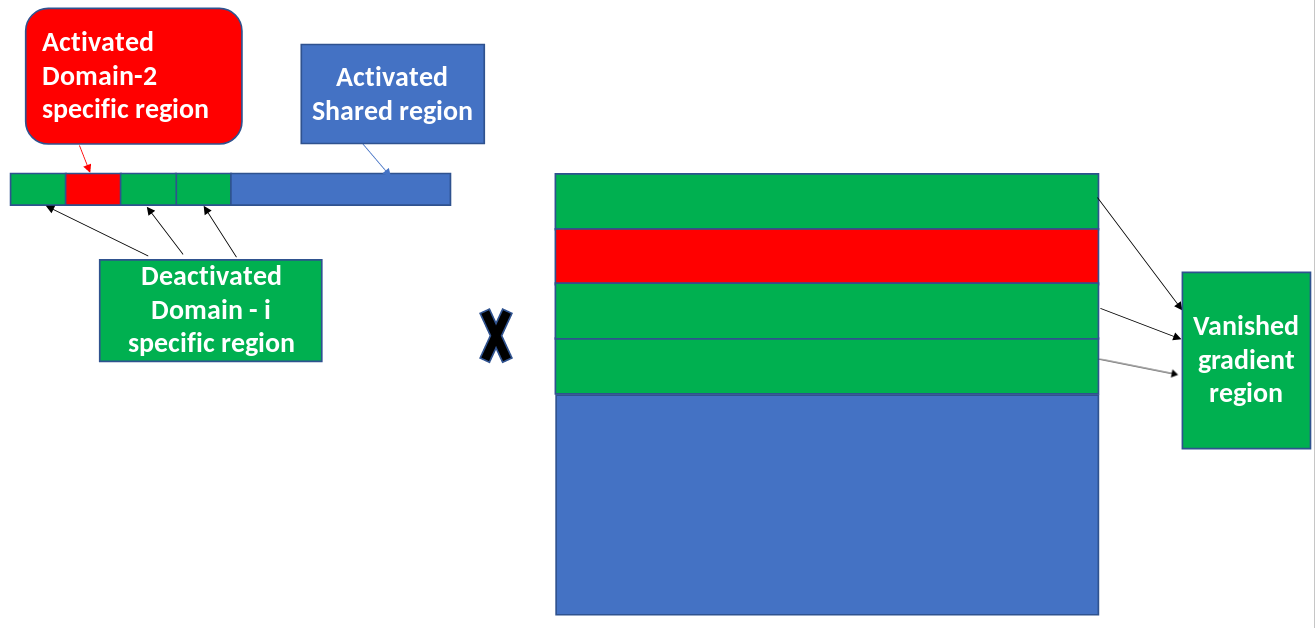
\includegraphics[width=0.8\linewidth]{Sparse1}
    \caption{Sparse word embeddings. The red region contains units that are activated only when an input from the corresponding domain is presented; the other (green) regions are deactivated; the blue (generic) region is always activated.} 
    \label{fig:network}
  \end{figure}
\fyTodo{Explain vanishing ?}
Figure~\ref{fig:network} presents our proposed design. During backprogation, the \Todo{rotation}{Why ?} matrix receives vanishing gradient at regions corresponding to deactivated regions in the word embedding. Those regions are also vanished in forward step, thus do not interfere the training on the domain to which they do not correspond.

Denote
$p_{t} = P * w_{t} = P_g \omega_g(t) + \displaystyle{\mathop{\sum}_{i \in [1,..,d]} P_i * \omega_i(t)}$\\
where $w_{t}$ is word embedding of token $x_{t}$  is projection of word embedding (Transformer \cite{NIPS2017_7181}, recurrent \cite{bahdanau2014neural})
Assume $x_{t}$ belongs to domain $i$, thus $w_j(t) = 0 \forall j \neq i$. Denote $P_j$ the rows of the projection matrix $P$ corresponding to the deactivated region $w_j$.
\begin{equation}
\begin{split}
\frac{\partial L(y_t,x_t)}{\partial P_j} &=\frac{\partial L}{\partial p}(p_t) * \frac{\partial p_t}{\partial P_j} \\
								&= \frac{\partial L}{\partial p}(p_t) * w_j(t)\\
									&=0
\end{split} 
\forall j \neq i
\end{equation}
\subsection{Implementation Details}
The complex structure of State-of-the-art architecture Transformer \cite{NIPS2017_7181} and popular recurrent network \cite{bahdanau2014neural} makes the implementation of sparse embedding non-obvious. Indeed, Transformer involve positional embedding and residual connections which are not homogeneous for domain-regions. Therefore, in our first implementation, we used an dense layer to fuse domain-region and generic region before applying positional embedding and residual connection. This implementation limits the finetuning effect at only word level.\\
Furthermore, because word embeddings are involved in three parts of standard encoder-decoder structure, which are input of encoder, input of decoder and projection before softmax, we have 7 possibilities to apply sparse embedding. However, due to high memory cost, we only want to apply sparse embedding on the source side. \fyTodo{Explain this. Future work ?}

\section{Experiments \label{sec:experiments}}

\subsection{Domains and data \label{ssec:data}}
To evaluate the performance of proposed architecture, we design experiments in which we want to train an NMT for 3 domains such as medical, administrative documents and business briefly denoted by EMEA, EPPS, ECB according to training corpora name respectively. We use 3 corpora for training: European Medicines Agency; European Central Bank and European Parliament \cite{Tiedemann2009RANLP5}. We randomly split those 3 corpora into training, validation and test set with size described in table \ref{table:Corpora}. We use validation sets for choosing the best model according to the average BLEU score on 3 validation sets. We also realize that the test sets origined from same corpora as training sets are likely easy for trained model, thus can not provide fair evaluation. Therefore, we we use Khresmoi-test; newstest2009 and test2007 for domains: EMEA, EPPS. Unfortunately, we could not find any official test sets for ECB domain. We also want to evaluate the generalization of trained model. The model is also required to achieve comparable performance to generic model. To do so, we use newstest 2009 and IWSLT 2010 whose contain does not particularly belong to any domain.\fyTodo{Clarify / simplify text}

\begin{table}[H]
\fyTodo{Too small ! Use abbrevs (En, Fr, ECB, EMEA, EPPS)}
  \resizebox{\columnwidth}{!}{
\begin{tabular}{ |l|l|l|l|l|l| }
\hline
Task & Corpora & Train & Dev & Test & Vocabulary \\ \hline
\multirow{5}{*}{$En \rightarrow Fr$} & European Medicines Agency & 1090568 & 1000 & 1000 & English: 30164, French: 30398\\
 & European Central Bank & 191960 & 1000 & 1000 &\\
 & European Parliament & 2005723 & 1000 & 1000 & \\ \hline
\multirow{5}{*}{$En \rightarrow Ge$} & European Medicines Agency & 1108752 & 1000 & 1000 & English: 30159, German: 30698\\
 & European Central Bank & 111174 & 1000 & 1000 &\\
 & European Parliament & 1920209 & 1000 & 1000 & \\ \hline
\hline
\end{tabular}
}
\caption{Corpora }
\label{table:Corpora}
\end{table}
\subsection{Baselines \label{ssec:baselines}}
\fyTodo{Describe baselines}

\subsection{NMT model configuration}
We evaluate our method on two state-of-the-art encoder-decoder architectures: a recurrent architecture based on attentional birectional Long Short-Term Memory (LSTM) cells and the Transformer architecture of \citet{NIPS2017_7181}.
More precisely, for the Transformer we use the same settings as described in \cite{NIPS2017_7181}. For the recurrent architecture, in order to fairly compare to the work of \citet{D18-1041}, we use a standard configuration with one layer bidirectional LSTM with a encoder hidden size of 1024; one attentional unidirectional LSTM layer with same hidden size in decoder; and word embeddings of size 512. The implementation can be found in OpenNMT-tf \cite{P17-4012}.
\fyTodo{Language pairs, BPE number, optimizer}
\fyTodo{Motivate the split}
For the implementation of sparse embeddings, we split the vector embedding of size 512 into four regions $[8,8,8,488]$, corresponding respectively to EMEA, EPPS, ECB domain and generic region. If sentence comes from domain $i$, regions for domains $j,\forall j \neq i$ will be masked as 0. We then use a dense layer of size 512 to fuse the active domain region and the generic region.

\begin{algorithm}[H]
\caption{Multi-domain Training}
\label{algo:1}
\begin{algorithmic}[1]
\REQUIRE {Corpora $C_i, i\in [1,..,d]$ for d domains}
\REPEAT 
\STATE{Randomly pick $i \in [1,..,d]$ w.r.t multinomial distribution $[\frac{|C_i|}{\displaystyle{\mathop{\sum}_{i\in [1,..,d]}|C_i|}}]$.}
\STATE{Randomly pick a batch of sentences from corpora $C_i$.}
\STATE{Activating only generic activate embedding to create generic embedding batch, denoted $W_g$}
\STATE{Pass the batch of word embedding to a dense layer to fuse regions}
\STATE{Computing gradient of $\theta_s$, $\frac{\partial L}{\partial \theta_s}$ using generic batch $W_g$}
\STATE{Activating corresponding domain region and generic region to create domain embedding batch}
\STATE{Pass the batch of word embedding to a dense layer to fuse regions.}
\STATE{Computing gradient of domain parameters $\theta_i$, $\frac{\partial L}{\partial \theta_i}$ using domain batch }
\STATE{Apply backprogation using computed gradients $\frac{\partial L}{\partial \theta_s}$ and $\frac{\partial L}{\partial \theta_i}$}
\UNTIL{convergence}
\end{algorithmic}
\end{algorithm}

Each iteration of algorithm \ref{algo:1}, the batch is doubled because it contains 2 types of word embedding for each sentence (using only generic region; using generic region and active domain region). The reason to do this is to minimize simultaneously both losses \\
$\theta^*_{s}=\displaystyle{\mathop{\argmin}_{\theta_s}}E_{(x,y) \sim D(\displaystyle{\mathop{\cup}_{i \in [1,..,d]}}C_{i})}[-log(p_{\theta_s}(y|x))]$ \\ 
$ \theta^*_{i}=\displaystyle{\mathop{\argmin}_{\theta_i}}E_{(x,y) \sim D(C_{i})}[-log(p_{\theta_i,\theta^*_s}(y|x,i))]
$ 
We admit that this is not the optimal way. However, this procedure makes training very simple.\fyTodo{Explain technicalities - future work ?}

We also take in account the problem of overfitting that could occur for small corpora. Indeed, real data are not always balanced for every domain. For instance, in our experiments, the size of corpora are very different where EPPS is largest with approximately 2 millions sentences, EMEA contains about 1 million sentences and ECB is the smallest with only 200 000 sentences for English French and 100 000 for English-German. If we train each corpora with same number of batches, ECB will be trained too oftenly, that easily leads to overfitting. Therefore, we perform backpropagation on corpora with frequencies according to sizes of corpora. \fyTodo{Refs on this ?}

\subsection{Results}
\begin{figure}[H]
\begin{center}
 \resizebox{\columnwidth}{!}{\begin{tabularx}{\textwidth}{|| X | X | X | X | X | X | X | X | X ||} 
 \hline
 Models & EMEA test & EPPS test & ECB test & khresmoi (EMEA domain) & test 2007 (EPPS domain) & newstest 2009 & newstest 2014 & IWSLT test 2010 \\ [0.5ex] 
 \hline\hline
 Mixed & 67.69 & 37.5 & 53.49 & 34.86 & 30.96 & 20.98 &  & 25.7 \\
 \hline
 EMEA-finetuned & 76.77 & 17.16 & 11.99 & 29.58 & 14.25 & 9.92 &  & 11.10 \\
 \hline
 EPPS-finetuned & 20.86 & 37.04 & 24.53 & 31.86 & 30.97 & 20.72 &  & 11.1 \\
 \hline
 ECB-finetuned & 9.2 & 18.39 & 55.45 & 12.13 & 16.12 & 8.71 &  & 7.19 \\
 \hline
 Sparse(1) & 70.45 & 38.23 & 54.69 & 34.66 & 31.24 & 21.36 & 28.12 & 26.02 \\
 \hline
 Sparse(2) & 69.91 & 38.05 & 54.2 & 35.22 & 31.25 & 21.36 & 28.12 & 26.02 \\
 \hline
 Sparse(3) &  &  &  &  &  &  &  & \\
 \hline
 Domain Control & 67.87 & 37.31 & 54.14 & 33.63 & 31.09 &  & & \\
 \hline
\end{tabularx}}
\end{center}
\caption{BPE-detokenized BLEU score in language pair English - French. Sparse(1) uses correponding domain tag for EMEA, EPPS, ECB test sets and generic tag for newstest and IWSLT. Sparse(2) uses generic tag for all of test sets. Sparse(3) uses tag predicted by pretrained domain classififer}
\label{tab:1}
\end{figure}

\begin{figure}[H]
\begin{center}
 \resizebox{\columnwidth}{!}{\begin{tabularx}{\textwidth}{|| X | X | X | X | X | X | X | X | X ||} 
 \hline
 Models & EMEA test & EPPS test & ECB test & khresmoi (EMEA domain) & test 2007 (EPPS domain) & newstest 2009 & newstest 2014 & IWSLT test 2010 \\ [0.5ex] 
 \hline\hline
 Mixed & 64.57 & 26.47 & 68.67 & 21.77 & 23.50 & 13.9 & 17.04 & 18.85 \\
 \hline
 EMEA-finetuned & & & & & & & & \\
 \hline
 EPPS-finetuned & & & & & & & & \\
 \hline
 ECB-finetuned & & & & & & & & \\
 \hline
 Sparse(1) & 70.55 & 26.17 & 68.07 & 21.50 & 23.30 & 14.05 & 16.64 & 19.04\\
 \hline
 Sparse(2) & 70.67 & 26.24 & 66.97 & & & 14.05 & 16.64 & 19.04 \\
 \hline
 Domain Control & & & & & & & & \\
 \hline
\end{tabularx}}
\end{center}
\caption{BLEU score for Transformer in language pair English - German. The notation is same as figure \ref{tab:1}}
\label{tab:2}
\end{figure}

\begin{figure}[H]
\begin{center}
 \resizebox{\columnwidth}{!}{\begin{tabularx}{\textwidth}{|| X | X | X | X | X | X | X | X | X ||} 
 \hline
 Models & EMEA test & EPPS test & ECB test & khresmoi (EMEA domain) & test 2007 (EPPS domain) & newstest 2009 & newstest 2014 & IWSLT test 2010 \\ [0.5ex] 
 \hline\hline
 Mixed & & & & & & & & \\
 \hline
 EMEA-finetuned & & & & & & & & \\
 \hline
 EPPS-finetuned & & & & & & & & \\
 \hline
 ECB-finetuned & & & & & & & & \\
 \hline
 Sparse & & & & & & & & \\
 \hline
 Domain Control & & & & & & & & \\
 \hline
 WDCMT (conditional GRU) & 68.76 & 35.71 & 52.75 & 32.03 & 29.81 & 19.58 & 24.63 & 23.28 \\
 \hline 
\end{tabularx}}
\end{center}
\caption{bpe-detokenized BLEU score for Recurrent network architecture on language pair English-French. Notations as same as figure \ref{tab:1} except that other models from WDCMT of \cite{D18-1041} use Bidirectional-LSTM}
\label{tab:3}
\end{figure}

\begin{figure}[H]
\begin{center}
 \resizebox{\columnwidth}{!}{\begin{tabularx}{\textwidth}{|| X | X | X | X | X | X | X | X ||} 
 \hline
 Models & EMEA test & EPPS test & ECB test & khresmoi (EMEA domain) & test 2007 (EPPS domain) & newstest 2009 & IWSLT test 2010 \\ [0.5ex] 
 \hline\hline
 Mixed & & & & & & & \\
 \hline
 EMEA-finetuned & & & & & & & \\
 \hline
 EPPS-finetuned & & & & & & & \\
 \hline
 ECB-finetuned & & & & & & & \\
 \hline
 Sparse & & & & & & & \\
 \hline
 Domain Control & & & & & & & \\
 \hline
 WDCMT (conditional GRU) & & & & & & & \\
 \hline 
\end{tabularx}}
\end{center}
\caption{BLEU score for Recurrent network on language pair English - German. Notations are the same as for figure~\ref{tab:3}}
\label{tab:4}
\end{figure}
\subsection{Word embedding analysis}

\section{Conclusions}
\fyTodo{natural continuations: go beyond words; learn the projection matrix at the word level; other ?}

\section*{Acknowledgments}
\fyTodo{Homegenize refs - urls, addresses, etc}
\bibliography{naaclhlt2019}
\bibliographystyle{plainnat}

\end{document}
